\chapter{Logic Circuits}\label{ch:logic}

\begin{objectives}
After studying this chapter you will be able to:
\begin{itemize}
  \item state the axioms, theorems and properties of Boolean algebra, including duality and De~Morgan's theorem, and prove them with truth tables;
  \item relate switching circuits to the AND, OR and NOT functions and draw the standard gate symbols;
  \item derive a canonical sum-of-products (SOP) or product-of-sums (POS) expression from a truth table using minterms and maxterms;
  \item simplify a Boolean expression algebraically and compare the cost of the original and simplified circuits;
  \item translate a word problem into a truth table, a Boolean expression, a logic network and a VHDL description; and
  \item verify a VHDL design with a simple testbench.
\end{itemize}
\end{objectives}

\section{Logic Circuits}
A \term{logic circuit} performs operations on digital signals. In a \term{binary logic circuit} each signal takes one of only two values, 0 or 1, which in an electronic circuit correspond to two voltage ranges (``low'' and ``high''). The most general form of a logic circuit is the \term{switching network} of \cref{fig:switching-network}: a block that accepts a set of discrete inputs $x_1,\dots,x_n$ and produces a set of discrete outputs $f_1,\dots,f_m$ that depend on those inputs.

\figw{179.2pt}{lect_2_switching_network}{A switching network: discrete inputs are transformed into discrete outputs.}{fig:switching-network}

If the outputs depend only on the \emph{present} values of the inputs the network is \term{combinational}; if they also depend on past inputs, the network is \emph{sequential} and must contain memory. This chapter and the next four deal with combinational networks; sequential circuits begin in \cref{ch:latches}.

\section{Boolean Algebra}\label{sec:boolean}
The mathematical tool used to describe and manipulate logic circuits is \term{Boolean algebra}. It was introduced by the English mathematician George Boole in \emph{An Investigation of the Laws of Thought} (1854)~\cite{boole1854}, where it was meant as an algebra of human reasoning rather than of circuits. The link to hardware was made by Claude Shannon in his 1938 master's thesis~\cite{shannon1938}, which showed that the algebra describes networks of relay switches exactly: a closed switch is 1 and an open switch is 0. Shannon's insight means that \emph{we can design digital circuits by doing mathematics}.

\subsection{Variables, operations and axioms}
A \term{Boolean variable} ($x$, $y$, $A$, \dots) may have only the value 0 or 1. These two symbols are \emph{not} ordinary numbers; they stand for two states, for example a low or a high voltage. Three operations are defined:
\begin{itemize}
  \item \term{AND} (logical product), written $x\cdot y$ or $xy$;
  \item \term{OR} (logical sum), written $x+y$; and
  \item \term{NOT} (complement or inversion), written $x'$ or $\NOT{x}$.
\end{itemize}
They are defined by the \term{axioms} of \cref{tab:axioms}. Note that $1+1=1$: the ``sum'' is a logical OR, not an arithmetic sum.

\begin{table}[htbp]
\centering
\caption{Axioms and single-variable theorems of Boolean algebra. Each line on the left is the \emph{dual} of the line on the right.}
\label{tab:axioms}
\renewcommand{\arraystretch}{1.2}
\begin{tabular}{@{}ll@{\qquad\qquad}ll@{}}
\toprule
\multicolumn{2}{c}{\textbf{Axioms}} & \multicolumn{2}{c}{\textbf{Single-variable theorems}}\\
\midrule
$0\cdot 0 = 0$ & $1+1 = 1$ & $x\cdot 0 = 0$ & $x+1 = 1$\\
$1\cdot 1 = 1$ & $0+0 = 0$ & $x\cdot 1 = x$ & $x+0 = x$\\
$0\cdot 1 = 1\cdot 0 = 0$ & $1+0 = 0+1 = 1$ & $x\cdot x = x$ & $x+x = x$\\
$x=0 \Rightarrow x'=1$ & $x=1 \Rightarrow x'=0$ & $x\cdot x' = 0$ & $x+x' = 1$\\
 & & \multicolumn{2}{c}{$(x')' = x$ \quad (involution)}\\
\bottomrule
\end{tabular}
\end{table}

\subsection{Properties of two and three variables}
The identities of \cref{tab:properties} are used continually to manipulate and simplify expressions. As in \cref{tab:axioms}, they come in dual pairs. Operator precedence follows ordinary algebra: NOT first, then AND, then OR, so $x + yz'$ means $x + (y\cdot(z'))$.

\begin{table}[htbp]
\centering
\caption{Properties of Boolean algebra.}
\label{tab:properties}
\renewcommand{\arraystretch}{1.25}
\begin{tabular}{@{}lll@{}}
\toprule
\textbf{Name} & \textbf{AND form} & \textbf{OR form}\\
\midrule
Commutative & $xy = yx$ & $x+y = y+x$\\
Associative & $x(yz) = (xy)z$ & $x+(y+z) = (x+y)+z$\\
Distributive & $x(y+z) = xy+xz$ & $x+yz = (x+y)(x+z)$\\
Absorption & $x(x+y) = x$ & $x+xy = x$\\
Combining (adjacency) & $(x+y)(x+y') = x$ & $xy+xy' = x$\\
De Morgan & $(x+y)' = x'y'$ & $(xy)' = x'+y'$\\
Consensus & $(x+y)(y+z)(x'+z) = (x+y)(x'+z)$ & $xy+yz+x'z = xy+x'z$\\
\bottomrule
\end{tabular}
\end{table}

\subsection{Duality}
\begin{definition}{Dual of an expression}{dual}
The \term{dual} of a Boolean expression is obtained by interchanging AND with OR and 0 with 1, leaving all variables (and complements) unchanged.
\end{definition}
\emph{Principle of duality:} if an equation is true, its dual is also true. For example, the dual of $x+0=x$ is $x\cdot 1=x$. This halves the work of learning the theorems, because every identity of \cref{tab:axioms,tab:properties} automatically yields a second one.

\subsection{De Morgan's theorem}
\term{De Morgan's theorem} gives the complement of a product or a sum:
\begin{equation}
  (xy)' = x' + y', \qquad (x+y)' = x'y'.
  \label{eq:demorgan}
\end{equation}
In words: the complement of an AND is the OR of the complements, and vice versa. The theorem extends to any number of variables, $(x_1x_2\cdots x_n)' = x_1'+x_2'+\cdots+x_n'$. It is the key to converting between SOP and POS forms and to implementing circuits with NAND or NOR gates (\cref{ch:kmap}).

\paragraph{Proof by perfect induction.} Because each variable takes only two values, an identity in $n$ variables can be proved by checking all $2^n$ combinations. For $(xy)'=x'+y'$:

\begin{center}
\begin{tabular}{cc|cc|cc|c}
\toprule
$x$ & $y$ & $xy$ & $(xy)'$ & $x'$ & $y'$ & $x'+y'$\\
\midrule
0&0&0&\textbf{1}&1&1&\textbf{1}\\
0&1&0&\textbf{1}&1&0&\textbf{1}\\
1&0&0&\textbf{1}&0&1&\textbf{1}\\
1&1&1&\textbf{0}&0&0&\textbf{0}\\
\bottomrule
\end{tabular}
\end{center}
The bold columns agree in every row, so the two sides are equal. The same result can be seen in the Venn diagrams of \cref{fig:venn}, where the shaded areas representing the two sides of the identities coincide.

\figw{272.2pt}{lect_2_venn}{Venn-diagram illustration of De Morgan's laws: the region shaded for the left-hand side equals that of the right-hand side.}{fig:venn}

\section{From Switches to Logic Functions}\label{sec:switches-logic}
The simplest binary element is a switch, and combinations of switches realise the basic functions.

\paragraph{AND: switches in series.} The lamp $L$ in \cref{fig:sw-and} lights only if $x_1$ \emph{and} $x_2$ are closed: $L(x_1,x_2) = x_1\cdot x_2$.

\paragraph{OR: switches in parallel.} In \cref{fig:sw-or} the lamp lights if $x_1$ \emph{or} $x_2$ (or both) is closed: $L(x_1,x_2) = x_1+x_2$.

\begin{figure}[htbp]
\centering
\begin{subfigure}[b]{201.3pt}\centering
  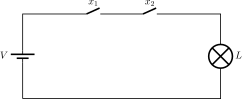
\includegraphics[width=199.3pt]{lect_2_switching_circuit_and}\caption{AND}\label{fig:sw-and}
\end{subfigure}
\hfill
\begin{subfigure}[b]{201.3pt}\centering
  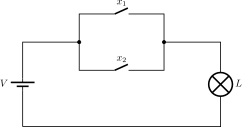
\includegraphics[width=199.3pt]{lect_2_switching_circuit_or}\caption{OR}\label{fig:sw-or}
\end{subfigure}
\\[6pt]
\begin{subfigure}[b]{158.8pt}\centering
  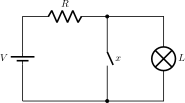
\includegraphics[width=156.8pt]{lect_2_switching_circuit_not}\caption{NOT}\label{fig:sw-not}
\end{subfigure}
\caption{Switching circuits for the three basic functions.}\label{fig:sw}
\end{figure}

\paragraph{NOT: a switch that diverts current.} Suppose the lamp should be on when the switch is \emph{open}. In \cref{fig:sw-not} current flows through the resistor $R$ and the lamp when switch $S$ is open ($x=0$); closing $S$ ($x=1$) short-circuits the lamp to ground. Hence $L = x'$.

\subsection{Truth tables}
A \term{truth table} lists the value of a function for every combination of its inputs; a function of $n$ variables has $2^n$ rows. The truth tables of the basic functions are in \cref{tab:basic-tt}. A truth table is the most complete and unambiguous specification of a combinational function, and it is the usual starting point of a design.

\begin{table}[htbp]
\centering
\caption{Truth tables of AND, OR and NOT.}
\label{tab:basic-tt}
\begin{tabular}{cc|c}
\toprule
$x_1$&$x_2$&$x_1x_2$\\ \midrule
0&0&0\\0&1&0\\1&0&0\\1&1&1\\ \bottomrule
\end{tabular}\qquad\qquad
\begin{tabular}{cc|c}
\toprule
$x_1$&$x_2$&$x_1+x_2$\\ \midrule
0&0&0\\0&1&1\\1&0&1\\1&1&1\\ \bottomrule
\end{tabular}\qquad\qquad
\begin{tabular}{c|c}
\toprule
$x$&$x'$\\ \midrule
0&1\\1&0\\ \bottomrule
\end{tabular}
\end{table}

\section{Logic Gates and Networks}\label{sec:gates}
Each basic operation is implemented by an electronic circuit called a \term{logic gate}, drawn with the standard symbols of \cref{fig:gate-symbols}. A gate has one or more inputs and one output. Gates are connected into a \term{logic network} (or logic circuit) that implements a larger function. For example, \cref{fig:logic-network} shows the function $f=(x_1+x_2)\cdot x_3$ realised by an OR gate feeding an AND gate.

\begin{figure}[htbp]
\centering
\begin{subfigure}[b]{138.7pt}\centering
  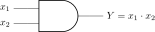
\includegraphics[width=136.7pt]{lect_2_and_symbol}\caption{AND}
\end{subfigure}
\hfill
\begin{subfigure}[b]{142.4pt}\centering
  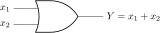
\includegraphics[width=140.4pt]{lect_2_or_symbol}\caption{OR}
\end{subfigure}
\hfill
\begin{subfigure}[b]{99.1pt}\centering
  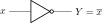
\includegraphics[width=97.1pt]{lect_2_not_symbol}\caption{NOT (inverter)}
\end{subfigure}
\caption{Graphical symbols of the basic gates.}\label{fig:gate-symbols}
\end{figure}

\figw{168.6pt}{lect_2_logic_network}{A logic network for $f=(x_1+x_2)\cdot x_3$: an OR gate feeding an AND gate.}{fig:logic-network}

\begin{lstlisting}[caption={VHDL description of $f=(x_1+x_2)\cdot x_3$.},label={lst:logic-function}]
library IEEE;
use IEEE.STD_LOGIC_1164.ALL;

entity logic_function is
  port (x1, x2, x3 : in  std_logic;
        f          : out std_logic);
end logic_function;

architecture behavioral of logic_function is
begin
  f <= (x1 or x2) and x3;
end behavioral;
\end{lstlisting}

\subsection{A first look at VHDL}
A hardware description language lets us write a circuit as text. A VHDL design unit has two parts, illustrated by \cref{lst:logic-function}.
\begin{itemize}
  \item The \code{entity} declares the \emph{interface}: the name of the circuit and its \code{port}s, each with a direction (\code{in} or \code{out}) and a type. We use \code{std_logic}, a one-bit type from the library \code{IEEE.std_logic_1164}.
  \item The \code{architecture} describes the \emph{behaviour} or structure. The statement \code{f <= (x1 or x2) and x3;} is a \term{concurrent signal assignment}: it describes a gate network that evaluates continuously, not a step executed once. Operators \code{and}, \code{or}, \code{not}, \code{xor}, \dots{} correspond directly to gates.
\end{itemize}
Appendix~\ref{app:vhdl} summarises the language elements used in this book.

\section{Logic Synthesis}\label{sec:synthesis}
\termx{Logic synthesis}{logic synthesis} is the process of producing a logic circuit that implements a desired function, usually given as a truth table or a Boolean expression. The primary goal is correctness; the secondary goal is optimisation: a circuit that is smaller, faster or uses less power. A function can be synthesised by looking at the rows where it is 1 or at the rows where it is 0, which leads to two standard forms.

\subsection{Sum of products and minterms}
A \term{minterm} of $n$ variables is a product (AND) term in which every variable appears exactly once, either complemented or not. Each minterm is 1 for exactly one row of the truth table, and the row number $i$ (read as a binary number) names the minterm $m_i$: a variable is complemented if its value in that row is 0 and uncomplemented if it is 1.

\begin{keypoint}[Synthesis of a sum of products]
(1)~Mark the rows in which $f=1$. (2)~Write the minterm of each marked row. (3)~OR the minterms together. The result is the \term{canonical sum of products} (canonical SOP), abbreviated $f=\Sm(\dots)$.
\end{keypoint}

\subsection{Product of sums and maxterms}
Dually, a \term{maxterm} is a sum (OR) term containing every variable once; it is 0 for exactly one row, and the maxterm $M_i$ is formed with a variable uncomplemented if its value in the row is 0 and complemented if it is 1. The \term{canonical product of sums} (canonical POS) ANDs the maxterms of all rows in which $f=0$: $f=\PM(\dots)$. Note that $m_i' = M_i$.

\begin{example}{SOP and POS of one function}{sop-pos}
The function $f(a,b,c)$ is 1 whenever $c=1$ (\cref{tab:sop-pos}).

\textbf{SOP:} the rows with $f=1$ are 1, 3, 5, 7, hence
\[
 f = a'b'c + a'bc + ab'c + abc = m_1+m_3+m_5+m_7 = \Sm(1,3,5,7).
\]
\textbf{POS:} the rows with $f=0$ are 0, 2, 4, 6, hence
\[
 f = (a+b+c)(a+b'+c)(a'+b+c)(a'+b'+c) = M_0M_2M_4M_6 = \PM(0,2,4,6).
\]
Both are correct and equal; in this case each simplifies to $f=c$.
\end{example}

\begin{table}[htbp]
\centering
\caption{Truth table of \cref{ex:sop-pos} with minterms and maxterms.}
\label{tab:sop-pos}
\begin{tabular}{ccc|c|ll}
\toprule
$a$&$b$&$c$&$f$&Minterm&Maxterm\\ \midrule
0&0&0&0&$m_0 = a'b'c'$&$\mathbf{M_0 = a+b+c}$\\
0&0&1&1&$\mathbf{m_1 = a'b'c}$&$M_1 = a+b+c'$\\
0&1&0&0&$m_2 = a'bc'$&$\mathbf{M_2 = a+b'+c}$\\
0&1&1&1&$\mathbf{m_3 = a'bc}$&$M_3 = a+b'+c'$\\
1&0&0&0&$m_4 = ab'c'$&$\mathbf{M_4 = a'+b+c}$\\
1&0&1&1&$\mathbf{m_5 = ab'c}$&$M_5 = a'+b+c'$\\
1&1&0&0&$m_6 = abc'$&$\mathbf{M_6 = a'+b'+c}$\\
1&1&1&1&$\mathbf{m_7 = abc}$&$M_7 = a'+b'+c'$\\
\bottomrule
\end{tabular}
\end{table}

\subsection{Minimality and simplification}
A canonical expression is seldom the cheapest. The cost of a circuit is roughly the number of gates and gate inputs, so we try to find an equivalent expression with fewer literals.

\begin{example}{Algebraic simplification}{simplify}
Simplify the canonical SOP $f(x_1,x_2) = x_1'x_2' + x_1'x_2 + x_1x_2$, whose truth table is 1, 1, 0, 1 for $x_1x_2 = 00, 01, 10, 11$.

\textbf{Solution.}
\begin{align*}
f &= x_1'(x_2'+x_2) + x_1x_2 && \text{(distributive)}\\
  &= x_1'\cdot 1 + x_1x_2 = x_1' + x_1x_2 && (x+x'=1)\\
  &= (x_1'+x_1)(x_1'+x_2) && \text{(distributive, OR form)}\\
  &= 1\cdot(x_1'+x_2) = x_1' + x_2 .
\end{align*}
The canonical form needs three 2-input AND gates, two inverters and a 3-input OR; the simplified form needs one inverter and one 2-input OR (\cref{fig:orig-simpl}).
\end{example}

\begin{figure}[htbp]
\centering
\begin{subfigure}[b]{215.4pt}\centering
  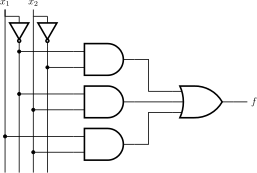
\includegraphics[width=213.4pt]{lect_2_sop_circuit}\caption{canonical form}
\end{subfigure}
\hfill
\begin{subfigure}[b]{147.2pt}\centering
  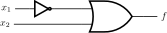
\includegraphics[width=145.2pt]{lect_2_simplified_circuit}\caption{simplified form $x_1'+x_2$}
\end{subfigure}
\caption{Two circuits for the same function of \cref{ex:simplify}.}\label{fig:orig-simpl}
\end{figure}

\Cref{lst:two-arch} shows an advantage of VHDL: one entity can have several architectures, so the unsimplified and simplified descriptions can be kept side by side and checked against each other in simulation. A particular architecture is selected by \emph{direct entity instantiation}, \code{UUT : entity work.Logic_Function(RTL_Simplified) port map (\dots);}, or by a \code{configuration} declaration.

\begin{lstlisting}[caption={One entity with two architectures: canonical and simplified.},label={lst:two-arch}]
library ieee;
use ieee.std_logic_1164.all;

entity Logic_Function is
  port (x1, x2 : in  std_logic;
        f      : out std_logic);
end entity Logic_Function;

-- canonical sum of products:  f = x1'x2' + x1'x2 + x1x2
architecture RTL_Canonical of Logic_Function is
begin
  f <= (not x1 and not x2) or (not x1 and x2) or (x1 and x2);
end architecture RTL_Canonical;

-- simplified:  f = x1' + x2
architecture RTL_Simplified of Logic_Function is
begin
  f <= not x1 or x2;
end architecture RTL_Simplified;
\end{lstlisting}

\section{Design Examples}\label{sec:examples2}
A systematic design proceeds from a word description to a truth table, to a Boolean expression, to a simplified expression and finally to a circuit and its VHDL description. We illustrate the flow with four examples.

\subsection{Three-way light control}
\begin{example}{Light controlled from three doors}{three-way}
A room has three doors, each with a switch $x_1,x_2,x_3$, that control a single light. Flipping any switch must toggle the light. When all switches are open (0) the light is off. Design the circuit.

\textbf{Truth table.} If one switch is closed the light is on; if two are closed it is off (flipping one switch from the one-closed state switched it off); if all three are closed it is on again. So $f=1$ in rows 1, 2, 4 and 7 (\cref{tab:threeway}).

\textbf{Expression.} The canonical SOP is
\[
 f = x_1'x_2'x_3 + x_1'x_2x_3' + x_1x_2'x_3' + x_1x_2x_3 .
\]
This is already the simplest SOP, but it has a compact form: $f$ is 1 when an \emph{odd} number of inputs is 1, which is the \term{exclusive OR} (XOR) of the three variables, $f = x_1\xor x_2\xor x_3$, where $x\xor y = x'y+xy'$.
\end{example}

\begin{table}[htbp]
\centering
\caption{Truth table for the three-way light.}
\label{tab:threeway}
\begin{tabular}{ccc|c}
\toprule
$x_1$&$x_2$&$x_3$&$f$\\ \midrule
0&0&0&0\\0&0&1&\textbf{1}\\0&1&0&\textbf{1}\\0&1&1&0\\
1&0&0&\textbf{1}\\1&0&1&0\\1&1&0&0\\1&1&1&\textbf{1}\\ \bottomrule
\end{tabular}
\end{table}

\Cref{lst:threeway} gives both descriptions and a testbench. The testbench is explained in \cref{sec:testbench}.

\begin{lstlisting}[caption={Three-way light: two architectures.},label={lst:threeway}]
library ieee;
use ieee.std_logic_1164.all;

entity three_way_light is
  port (x1, x2, x3 : in  std_logic;
        f          : out std_logic);
end three_way_light;

-- direct sum of products
architecture arch_sop of three_way_light is
begin
  f <= (not x1 and not x2 and x3) or (not x1 and x2 and not x3) or
       (x1 and not x2 and not x3) or (x1 and x2 and x3);
end arch_sop;

-- XOR form: same function, simpler description
architecture arch_simplified of three_way_light is
begin
  f <= x1 xor x2 xor x3;
end arch_simplified;
\end{lstlisting}

\subsection{Two-to-one multiplexer}
\begin{example}{Multiplexer}{mux}
Design a circuit that selects between two data inputs $x_1$ and $x_2$ using a control input $s$: $f=x_1$ if $s=0$ and $f=x_2$ if $s=1$.

\textbf{Truth table.} Rows are ordered $s\,x_1x_2$ (\cref{tab:mux}). $f=1$ in rows 2, 3, 5 and 7.

\textbf{Expression and simplification.}
\begin{align*}
f &= s'x_1x_2' + s'x_1x_2 + sx_1'x_2 + sx_1x_2\\
  &= s'x_1(x_2'+x_2) + sx_2(x_1'+x_1) = s'x_1 + sx_2 .
\end{align*}
The circuit is two AND gates, one inverter and one OR gate (\cref{fig:mux}).
\end{example}

\begin{table}[htbp]
\centering
\caption{Truth table of a 2-to-1 multiplexer.}
\label{tab:mux}
\begin{tabular}{ccc|c}
\toprule
$s$&$x_1$&$x_2$&$f$\\ \midrule
0&0&0&0\\0&0&1&0\\0&1&0&\textbf{1}\\0&1&1&\textbf{1}\\
1&0&0&0\\1&0&1&\textbf{1}\\1&1&0&0\\1&1&1&\textbf{1}\\ \bottomrule
\end{tabular}
\end{table}

\begin{figure}[htbp]
\centering
\begin{subfigure}[b]{223.9pt}\centering
  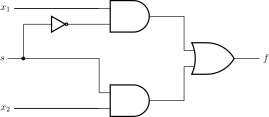
\includegraphics[width=221.9pt]{lect_2_mux_2to1}\caption{circuit for $f=s'x_1+sx_2$}
\end{subfigure}
\hfill
\begin{subfigure}[b]{75.3pt}\centering
  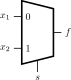
\includegraphics[width=73.3pt]{lect_2_mux_2_to_1_symbol}\caption{graphical symbol}
\end{subfigure}
\caption{A 2-to-1 multiplexer. The multiplexer is one of the most useful blocks in digital design and is studied further in \cref{ch:blocks}.}\label{fig:mux}
\end{figure}

\subsection{Car safety alarm}
\begin{example}{Car alarm}{car-alarm}
A car alarm $A$ must sound if (1)~the key is in the ignition ($K=1$) and the door is not closed ($D=0$), or (2)~the door is closed ($D=1$), the key is in ($K=1$), the driver is in the seat ($S=1$) and the seat belt is not fastened ($B=0$). Derive a minimal expression.

\textbf{Solution.} Translating the conditions, $A = KD' + DKSB'$. Factor out $K$: $A = K(D' + DSB')$. Using the identity $X + X'Y = X+Y$ (proved by distributing: $X+X'Y=(X+X')(X+Y)=X+Y$) with $X=D'$,
\[
  A = K\,(D' + SB').
\]
This needs one inverter for $D$, one for $B$, one AND, one OR and one more AND (\cref{fig:car-alarm}), far fewer than the original expression, and the VHDL is a single line, \cref{lst:car-alarm}.
\end{example}

\begin{figure}[htbp]
\centering
\begin{subfigure}[b]{130.2pt}\centering
  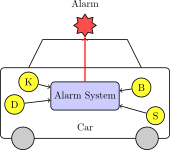
\includegraphics[width=128.2pt]{lect_2_car_alarm_sketch}\caption{the system}
\end{subfigure}
\hfill
\begin{subfigure}[b]{239.3pt}\centering
  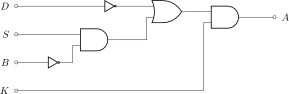
\includegraphics[width=237.3pt]{lect_2_car_alarm}\caption{circuit for $A=K(D'+SB')$}
\end{subfigure}
\caption{The car safety alarm of \cref{ex:car-alarm}.}\label{fig:car-alarm}
\end{figure}

\begin{lstlisting}[caption={Car alarm logic.},label={lst:car-alarm}]
library ieee;
use ieee.std_logic_1164.all;

entity car_alarm_logic is
  port (K, D, S, B : in  std_logic;
        A          : out std_logic);
end entity car_alarm_logic;

architecture rtl of car_alarm_logic is
begin
  A <= K and (not D or (S and not B));     -- A = K (D' + S B')
end architecture rtl;
\end{lstlisting}

\subsection{Half adder}
\begin{example}{Half adder}{half-adder}
Design a circuit that adds two bits $x$ and $y$ and produces a \emph{sum} bit $s$ and a \emph{carry} bit $c$.

\textbf{Truth table.} The arithmetic $0{+}0=00$, $0{+}1=01$, $1{+}0=01$, $1{+}1=10$ gives \cref{tab:ha}. The sum is 1 only when the inputs differ, so $s = x'y+xy' = x\xor y$; the carry is 1 only when both inputs are 1, so $c = xy$.
\end{example}

\begin{table}[htbp]
\centering
\caption{Half adder.}
\label{tab:ha}
\begin{tabular}{cc|cc}
\toprule
$x$&$y$&sum $s$&carry $c$\\ \midrule
0&0&0&0\\0&1&1&0\\1&0&1&0\\1&1&0&1\\ \bottomrule
\end{tabular}
\end{table}

The circuit is an XOR gate and an AND gate (\cref{fig:ha}). The half adder is the starting point of the arithmetic circuits of \cref{ch:arith}.

\begin{figure}[htbp]
\centering
\begin{subfigure}[b]{179.5pt}\centering
  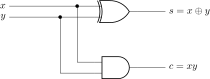
\includegraphics[width=177.5pt]{lect_2_half_adder}\caption{gate-level circuit}
\end{subfigure}
\hfill
\begin{subfigure}[b]{183.3pt}\centering
  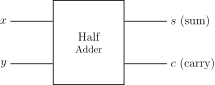
\includegraphics[width=181.3pt]{lect_2_half_adder_block}\caption{block diagram}
\end{subfigure}
\caption{Half adder.}\label{fig:ha}
\end{figure}

\begin{lstlisting}[caption={Half adder in VHDL (dataflow style).},label={lst:half-adder}]
library ieee;
use ieee.std_logic_1164.all;

entity half_adder is
  port (x, y : in  std_logic;     -- the two bits to add
        s, c : out std_logic);    -- sum and carry-out
end entity half_adder;

architecture dataflow of half_adder is
begin
  s <= x xor y;                   -- sum
  c <= x and y;                   -- carry
end architecture dataflow;
\end{lstlisting}

\section{The VHDL Testbench}\label{sec:testbench}
A \term{testbench} is a VHDL entity used to simulate and check another entity, the \emph{unit under test} (UUT). A testbench has no ports because it is closed: it generates its own stimulus and observes the UUT's response (\cref{fig:tb}). Writing a testbench takes four steps.
\begin{enumerate}
  \item \textbf{Instantiate} the UUT as a \code{component} (or by direct entity instantiation) and connect its ports to local signals.
  \item \textbf{Generate stimulus.} A \code{process} assigns values to the input signals and uses \code{wait for} statements to advance simulated time.
  \item \textbf{Observe} the outputs in the simulator's waveform window.
  \item \textbf{Verify.} Compare the waveform with the truth table, either by inspection or automatically with \code{assert} statements that report an error if an output is wrong.
\end{enumerate}

\figw{265.8pt}{lect_2_test_bench}{The relationship between a testbench and the unit under test (UUT).}{fig:tb}

\begin{lstlisting}[caption={A testbench for the three-way light that applies all eight input combinations.},label={lst:tb}]
library ieee;
use ieee.std_logic_1164.all;

entity three_way_light_tb is end entity;          -- no ports

architecture behavior of three_way_light_tb is
  signal x1, x2, x3 : std_logic := '0';            -- inputs to the UUT
  signal f          : std_logic;                   -- output of the UUT
begin
  uut : entity work.three_way_light(arch_simplified)
        port map (x1 => x1, x2 => x2, x3 => x3, f => f);

  stim_proc : process
  begin
    wait for 100 ns;                               -- let the simulator settle
    x1<='0'; x2<='0'; x3<='0'; wait for 10 ns;     -- expect f = 0
    x1<='0'; x2<='0'; x3<='1'; wait for 10 ns;     -- expect f = 1
    x1<='0'; x2<='1'; x3<='0'; wait for 10 ns;     -- expect f = 1
    x1<='0'; x2<='1'; x3<='1'; wait for 10 ns;     -- expect f = 0
    x1<='1'; x2<='0'; x3<='0'; wait for 10 ns;     -- expect f = 1
    x1<='1'; x2<='0'; x3<='1'; wait for 10 ns;     -- expect f = 0
    x1<='1'; x2<='1'; x3<='0'; wait for 10 ns;     -- expect f = 0
    x1<='1'; x2<='1'; x3<='1'; wait for 10 ns;     -- expect f = 1
    wait;                                          -- stop the process
  end process;
end architecture behavior;
\end{lstlisting}

\Cref{fig:sim-threeway} shows the waveform obtained by simulating \cref{lst:tb} in the Intel\textregistered\ Questa simulator. Each of the eight 10~ns intervals corresponds to one row of \cref{tab:threeway}; the output $f$ is high in rows 1, 2, 4 and 7, as predicted.

\begin{figure}[htbp]
\centering
\wavesplit{lect_2_three_way_light_sim}{4}
\caption{Simulation of the three-way light in Intel Questa (author's screenshot).}\label{fig:sim-threeway}
\end{figure}

\begin{caution}
Writing the expected value of $f$ only by looking at the simulation output proves nothing: the simulator will always give you the answer your design computes. Work out the expected outputs from the truth table \emph{first}, then compare.
\end{caution}

\begin{chaptersummary}
\begin{itemize}
  \item \textbf{Boolean algebra} has two values and three operations (AND, OR, NOT). Its theorems appear in dual pairs; \textbf{De Morgan's theorem} gives the complement of a sum or a product.
  \item An identity can be proved by \textbf{perfect induction}: check every row of the truth table.
  \item A \textbf{truth table} fully specifies a combinational function. \textbf{Gates} implement the basic operations and are connected into \textbf{logic networks}.
  \item A function with $f=1$ in rows $i_1,i_2,\dots$ has the canonical \textbf{SOP} $\Sm(i_1,i_2,\dots)$; with $f=0$ in rows $j_1,\dots$ it has the canonical \textbf{POS} $\PM(j_1,\dots)$.
  \item \textbf{Simplification} reduces the number of gates and inputs; the same function may have many equivalent expressions.
  \item The design flow is: \emph{word problem $\to$ truth table $\to$ expression $\to$ simplification $\to$ circuit $\to$ VHDL $\to$ testbench}.
  \item A VHDL \textbf{entity} defines the interface and an \textbf{architecture} the behaviour; a \textbf{testbench} stimulates the unit under test and lets us check it against the truth table.
\end{itemize}
\end{chaptersummary}

\chapsec{Exercises}
\begin{exlist}
  \item \textbf{Majority function.} A majority function is true when more than half of its inputs are true. (a)~Write the truth table of a 3-input majority function $f(x,y,z)$. (b)~Write its canonical SOP. (c)~Simplify it algebraically. (d)~Draw the circuit using AND, OR and NOT gates. (e)~Write VHDL and a testbench that applies all eight input combinations, and show the waveform.
  \item \textbf{Home alarm.} The alarm $A$ sounds if the system is armed ($S=1$) \emph{and} either the front door ($D=1$) or the window ($W=1$) is open. It never sounds if the system is not armed. Give the truth table, the Boolean expression, the circuit, and a simulation of the case $S=1$, $D=1$.
  \item \textbf{Line-following robot.} A robot has three sensors $L$, $C$, $R$ (value 0 over the black line, 1 over the white surface) and two motors $M_L$, $M_R$. It must \emph{go forward} ($M_L=M_R=1$) when centred ($L=1,C=0,R=1$); \emph{turn right} ($M_L=1, M_R=0$) when it drifts left ($L=1,C=1,R=0$); \emph{turn left} ($M_L=0,M_R=1$) when it drifts right ($L=0,C=1,R=1$); and \emph{stop} ($M_L=M_R=0$) in every other case. (a)~Write the truth table. (b)~Write SOP expressions for $M_L$ and $M_R$ and simplify them. (c)~Draw the circuits. (d)~Simulate all four behaviours.
  \item \textbf{Seven-segment decoder.} A seven-segment display has segments $a,b,c,d,e,f,g$ (\cref{fig:sevenseg}). Design a decoder with a 4-bit BCD input $b_3b_2b_1b_0$ that lights the segments to show the digits 0--9. Assume a \emph{common anode} display, in which a segment lights when its control signal is \emph{low}. (a)~Give the truth table, treating the input values 10--15 as don't-cares. (b)~Find the simplified SOP for segment $a$ (you may postpone the other segments until you have learnt Karnaugh maps in \cref{ch:kmap}). (c)~Draw the circuit for segment $a$.
  \item Use truth tables to prove: (a)~$x+xy=x$; (b)~$x+yz=(x+y)(x+z)$; (c)~$xy+x'z+yz=xy+x'z$.
  \item Write the dual of each identity: (a)~$x+x'y=x+y$; (b)~$(x+y)(x+z)=x+yz$; (c)~$xy+x'z+yz = xy+x'z$.
  \item Use De Morgan's theorem to find the complement of each function and express it as a sum of products: (a)~$F=x+yz'$; (b)~$F=x'y+xy'$; (c)~$F=(a+b)(c+d)$.
  \item Simplify algebraically, stating the identity used in each step: (a)~$F=x'y+xy+x'y'$; (b)~$F=(x+y)(x+y')(x'+z)$; (c)~$F=xy+x'z+yz$.
  \item A function is defined by $f=\Sm(0,3,5,6)$ of three variables $x,y,z$. (a)~Write the canonical SOP and the canonical POS. (b)~Describe in words when $f=1$. (c)~Give the complement $f'$ in $\Sm$ notation.
  \item Design a circuit with inputs $x_1,x_2,x_3$ whose output is 1 if and only if \emph{exactly two} of the inputs are 1. Give the canonical SOP and draw the circuit.
  \item Design a circuit with two 2-bit inputs $A=A_1A_0$ and $B=B_1B_0$ whose output $E$ is 1 when $A=B$. \emph{Hint:} $A=B$ if and only if each pair of corresponding bits is equal, and two bits are equal when their XOR is 0.
  \item How many different Boolean functions exist of (a)~two variables; (b)~three variables; (c)~$n$ variables? \emph{Hint:} each function is defined by a column of the truth table.
  \item The three-way light of \cref{ex:three-way} is extended to a corridor with four switches $x_1,\dots,x_4$, each of which toggles the light. (a)~Write the function using XOR. (b)~How many minterms does the canonical SOP contain?
\end{exlist}

\begin{figure}[htbp]
\centering
\begin{tikzpicture}[x=1cm,y=1cm]
  \tikzset{seg/.style={fill=kmutnborange!85, draw=none}, lab/.style={font=\sffamily\scriptsize}}
  \fill[seg] (0.15,2.35) -- (0.35,2.55) -- (1.65,2.55) -- (1.85,2.35) -- (1.65,2.15) -- (0.35,2.15) -- cycle;
  \fill[seg] (0.1,1.1) -- (0.3,1.3) -- (0.3,2.1) -- (0.1,2.3) -- (-0.1,2.1) -- (-0.1,1.3) -- cycle;
  \fill[seg] (1.9,1.1) -- (2.1,1.3) -- (2.1,2.1) -- (1.9,2.3) -- (1.7,2.1) -- (1.7,1.3) -- cycle;
  \fill[seg] (0.15,1.05) -- (0.35,1.25) -- (1.65,1.25) -- (1.85,1.05) -- (1.65,0.85) -- (0.35,0.85) -- cycle;
  \fill[seg] (0.1,-0.1) -- (0.3,0.1) -- (0.3,0.8) -- (0.1,1.0) -- (-0.1,0.8) -- (-0.1,0.1) -- cycle;
  \fill[seg] (1.9,-0.1) -- (2.1,0.1) -- (2.1,0.8) -- (1.9,1.0) -- (1.7,0.8) -- (1.7,0.1) -- cycle;
  \fill[seg] (0.15,-0.15) -- (0.35,0.05) -- (1.65,0.05) -- (1.85,-0.15) -- (1.65,-0.35) -- (0.35,-0.35) -- cycle;
  \node[lab] at (1,2.85) {a}; \node[lab] at (2.45,1.7) {b}; \node[lab] at (2.45,0.45) {c};
  \node[lab] at (1,-0.7) {d}; \node[lab] at (-0.45,0.45) {e}; \node[lab] at (-0.45,1.7) {f}; \node[lab] at (1,1.45) {g};
\end{tikzpicture}
\caption{Segment labels of the seven-segment display used in Exercise~2.4.}
\label{fig:sevenseg}
\end{figure}

\chapsec{Further Reading}
The reader who wants a systematic treatment of Boolean algebra and switching functions will find it in Brown and Vranesic~\cite{brown2009} and in Mano and Ciletti~\cite{mano2018}; Wakerly~\cite{wakerly2006} gives a particularly careful account of the relation between gates, expressions and timing. Shannon's thesis~\cite{shannon1938} remains very readable. For VHDL, see Ashenden~\cite{ashenden2008} and the language standard~\cite{ieee1076}.
